\chapter{Software OpenSource y Libre}
		\subsection{Introdución} 
Una interpretación de lo que se entiende por el término \textit{open source}, cuando se utiliza en el contexto de la descripción de un programa de software o diseño de hardware, es que el código fuente del diseño se encuentra disponible a la vista de alguna forma. A pesar de que es una amplia y potencialmente término ambiguo , un común acuerdo sobre la definición está en un documento llamado la Open Source Definition (OSD ), publicado por la Open Source Initiative (OSI).
Una interpretación sencilla de lo que se entiende por el término open source , cuando se utiliza en el contexto de la descripción de un programa de software o diseño de hardware , es que el diseño Fuentes de alguna manera están disponibles a la vista. A pesar de que es un amplio y potencial término ambiguo, un común acuerdo sobre la definición está en un documento llamado  Open Source Definition (OSD ), publicado por la Open Source Initiative (OSI).

La definición no es una licencia de software libre en sí, si no algo para medir condiciones frente a la distribución para determinar si cumplen y, si lo hacen, entonces se puede decir que es \textit{open source}\cite{Etiqueta06}.La definición no es una licencia de software libre en sí, si no algo para medir condiciones frente a la distribución para determinar si cumplen y, si lo hacen, entonces se puede decir que es \textit{open source}. Cuando el software \textit{libre} o \textit{free} se utiliza para describir el software de código abierto, se refiere a los derechos y no al costo del usuario. La Fundación para el Software Libre (FSF) ofrece una definición para mostrar claramente qué se tiene que cumplir sobre el software para que pueda ser considerado libre \cite{Etiqueta07}. El termino Free Software Foundation (FOSS) es usado para referirse al software que se adhiere al OSD y FSF. El software libre y de código abierto es una sociedad inclusiva término que abarca tanto el software libre y software de código abierto que a pesar de describir modelos de desarrollo similares, tienen diferentes culturas y filosofías.

El software \textit{libre} se refiere a la libertad de los usuarios para ejecutar, copiar, distribuir, estudiar, cambiar y mejorar el software. El vocablo \textit{free} en ingles significa :gratis y/o libre. Por ello el término ha ocasionado confusiones dándose a entender, equivocadamente, que el software libre es gratuito o regalado. Pero no es una cuestión de presencia o ausencia de costo, puesto que el software libre no significa que no pueda ser comercial.

Stallman fundó la Free Software Foundation (FSF ) en 1985 para promover la libertad del usuario y para defender los derechos de todo el software libre\cite{Etiqueta14}. La FSF patrocina el proyecto GNU. El software libre permite al usuario el ejercicio de cuatro libertades básicas:

\begin {itemize}
\item
 \textit{Libertad 0} Además el software \textit{libre} permite estudiar cómo funcionan y adaptarlo a las necesidades de quien lo use. Tener acceso a su código fuente posibilita, entre otras cosas, descubrir qué posibilidades tiene, etc. El adaptar el programa a las necesidades del usuario se puede suprimir partes que no le interesen, agregar otras partes que considere importantesm copiar una parte que realiza una tarea y/o adicinarla a otro programa, etc.

\item
\textit{Libertad 1} El software, sus copias y las modificaciones se pueden distribuir libremente, lo que significa poseer la libertad de redistribuir el programa, gratis o con algún costo, ya sea por mail, FTP, o en CD, redistibuyéndolo a una persona o a varias, a una persona que vive en otro país, etc.

\item 
\textit{Libertad 2} Es posible mejorarlo y hacer pública esas mejoras. La libretad de hacer un programa mejor, implica que se puede hacer menores los requerimientos de hardware para funcionar, que tenga mayores prestaciones, que sus requerimientos no sean tan altos, que tenga menos errores, etc. El poder liberar las mejoras al público quiere decir que si se realiza una mejora que permita un requerimiento menor de hardware, o que haga que ocupe menos espacio, se puede redistribuir ese programa mejorando o simplenete propoenr la mejora en lugar público (un foro de noticias, una lista de correo, un sitio web, un FTP, un canal de chat).

\item 
\textit{Libertad 3} El usuario al poseer el código fuente tiene poder de decisón, ya que podrá elegir quién puede modifica los programas que ha adquirido para mejorarlos (o bien mejorarlos el mismo). Es decir esto permite que no exista un monopolio, porque en el caso de que un software sea discontinuado el usuario podrá nuevamente (al poseer el código) elegir a un desarrollador para continuar utilizando el software que fue discontinuado. Además el usuario no estará completamente a merced de tener que renovar su hardware y software constantemente según ocurre a menudo con las políticas de las empresas que producen software privativo y también será libre de vender o redistribuir software libre.
 
 \end {itemize}
 
Mediante la licencias un autor permite el uso de su creación a otras personas, de la manera que el cree aceptable. En ese sentido la licencia es el instrumento que regula las maneras en que el usuario puede utilizar el software.

También una licencia de software es un contrato que determina en qué condiciones el usuario puede utilizar el programa informático y qué obligaciones asquiere para su uso. Cuando se instala un programa informático, o a veces, incluso, por el simple hecho de abrir el sobre que lo contiene, se esta aceptando las condiciones de su licencia de software.

Cuando IBM comenzó la venta de computadoras a gran escala en la década de 1960, el software venia incluido como código fuente. Una década más tarde, sin embargo, comenzaron a "desagregar"  el software, y se convirtió en habitual para los fabricantes de computadoras, no solo limito  el uso del mismo código fuente a los competidores, sino que también elimino la capacidad de modificar el código libremente y compartirlo \cite{Etiqueta08}.  
	
La licencia División de Software de Berkeley (BSD) y la Pública General del proyecto GNU (GNU GPL) son dos de las primeras licencias de código abierto. Ambos proporcionan la libertad de usar software de código fuente abierto para cualquier propósito y permitir la modificación y la distribución de su código fuente sin tener que pagar regalías. Las diferencias entre los dos pone de relieve una diferencia ideológica entre los defensores del código abierto .

Un punto significativo de diferencia entre las licencias BSD y GPL es que este último le permite
\textit{modificar su copia o copias del Programa o cualquier parte de el, y copie
y distribuir tales modificaciones ... supuesto que además ... hace que la
totalidad de cualquier trabajo que distribuya o publique y que en todo o en
parte contenga el Programa o cualquier parte del mismo, ya sea con o sin
modificaciones, para ser autorizadas sin cargo alguno para terceras partes bajo el
términos de esta Licencia Pública General.(GPLv1).} \cite{Etiqueta09}

La GNU GPL se conoce como una licencia \textit{viral}, en que cualquier diseño haciendo uso de código ya licenciado bajo la GNU GPL debe ser entonces licenciado bajo la
GNU GPL o cualquier licencia juzgados como igualmente sin restricciones por la FSF. En pocas palabras, una condición de uso del código licenciado bajo GPL es que su diseño se debe tener licencia bajo la GPL o una licencia compatible. Las licencias que se consideran compatibles con la GPL por la FSF son generalmente similares en las libertades que garantiza el software libres. La licencia se transmite al código que hacen uso de ella. El GNU GPLv3 exige que cuando un proyecto adopta esta licencia el código fuente debe estar disponible y que las patentes o derechos digitales (DRM) no inhiben a otros del uso del diseño. 

La licencia BSD modificada es básicamente la misma que la original sin la clausula de publicidad. De acuerdo con dicha cláusula, todo el material de publicidad en el cual se menciona características o la utilización de este software tenia que mostrar el siguiente asentimiento:"este producto incluye software desarrollado por la Universidad de California, Berkeley y sus contribuyentes ".

Esta cláusula de publicidad no permitía que fuera compatible con la lincencia GPL pero a partir de su versión 2.0 fue eliminada y la licencia pasó a ser compatible con la GPL.

La GNU GPL es en cierto modo, más restrictiva que la licencia BSD sobre las libertad de hacer lo que uno quiere con el código fuente. En la GNU se estipula que el código modificado debe estar disponible, y cualquier diseño utilizado con código GPL tiene también que venir bajo la GNU GPL. Sin embargo, esto no es diferente a cualquier licencia comercial, donde el código fuente escrito por un empleado de una empresa,o todo el código que se modifican o crean esta bajo la licencia exclusiva de la empresa. En el caso de la licencia de GNU, sin embargo, los usuarios están obligados a mantener su diseño abierto y libre como la GPL de GNU hace, de la misma manera el empleado de la empresa está obligado a mantener su código propietario en secreto para cualquiera que no sea de la  empresa.

Otro punto de controversia es el uso combinado de los diseños en los que cada uno esta bajo una licencia diferente, dando lugar al concepto de \textit{compatibilidad de la licencia}. En el caso de que un diseño utilizara una librería bajo licencia GPL, la GNU GPL especifica que se puede utilizar si el diseño  que requiere la librería este también bajo la GPL. 

 Una solución para aquellos que deseen escribir bibliotecas, y no tienen la
interpretación más estricta de la trabajos derivados se les aplica la propuesta de el  Proyecto GNU la Licencia Pública General Reducida de GNU, o más conocida por su nombre en inglés GNU Lesser General Public License (antes GNU Library General Public License o Licencia Pública General para Bibliotecas de GNU),o simplemente por su acrónimo del inglés GNU LGPL, esta licencia permisiva se aplica a cualquier programa o trabajo que contenga una nota puesta por el propietario de los derechos del trabajo estableciendo que su trabajo puede ser distribuido bajo los términos de esta "LGPL Lesser General Public License". El "Programa", utilizado en lo subsecuente, se refiere a cualquier programa o trabajo original, y el "trabajo basado en el Programa" significa ya sea el programa o cualquier trabajo derivado del mismo bajo la ley de derechos de autor: es decir, un trabajo que contenga el Programa o alguna porción de él, ya sea íntegra o con modificaciones o traducciones a otros idiomas.
Otras actividades que no sean copia, distribución o modificación no están cubiertas en esta licencia y están fuera de su alcance. El acto de ejecutar el programa no está restringido, y la salida de información del programa está cubierta sólo si su contenido constituye un trabajo basado en el Programa (es independiente de si fue resultado de ejecutar el programa). Si esto es cierto o no depende de la función del programa.\cite{Etiqueta03}

Estas diferencias de opinión con respecto a lo que constituye una obra derivada, y
la ambigüedad en torno a otros aspectos de la concesión de licencias de código abierto podría tener consecuencias para campos como el diseño de hardware y se discutirá en una sección posterior.

La principal diferencia de opinión, sin embargo , se deriva del hecho de que la libre
Software Foundation desean hacer imposible que el software propietario  pueda utilizar
software liberado bajo la GNU GPL. La FSF argumenta  que los que no están dispuesto a permitir que otras personas vean o modificar libremente su código aprovechen de los que si lo permiten. Otras licencias de código abierto, sin embargo ,son más permisivas en la utilización de sus diseños como por ejemplo en el codigo fuente de las librerias, en aplicaciones propietarias.

El objetivo del Proyecto GNU de implementar un sistema operativo completamente libre y gratuito, avanzo a buen ritmo en la década del 90, pero le faltaba la lleve de componentes del nivel más bajo.

El núcleo Linux iniciado por Linus Torvalds, fue liberado para poder ser modificado libremente en 1991. La licencia inicial, no fue exactamente una licencia d software libre, sin embargo la version 0.12 lanzada en febrero de 1992, fue licenciada nuevamente por Torvalds bajo los términos de la licencia pública general de GNU. Así como Unix en su tiempo, el núcleo de Torvalds atrajo la atención de programadores voluntario.

Hasta este punto, la falta de núcleo del proyecto GNU significaba la no existencia de un sistema operativo libre completo. El desarrollo de núcleo de Linux Torvalds lleno este último hueco. La conbinación del casi terminado sistema operativo GNU y el núcleo LInux resultó en el primer sistema operativo completo de softwore libre.

Entre las distribuciones Linux, Debian GNU/Linux, iniciada por Ian Murdock en 1993, es notorio por estar comprometido explicitamente con los prinicipios de GNU y la FSF del softwore libre. Los principios de desarrolladores de Debian estan expresados en el contrato social de Debian. Desde sus inicios, el proyecto de Debian ha estado intimamente ligado con la FSF, y de hecho fue patrocinado por la FSF durante un año. Sin embargo Debian ya no se considera software libre por la FSF y el proyecto GNU ya que el núcleo Linux incluido con Debian contiene partes privativas ademas de ofrecer repositorios con software no libre %\cite{Etiqueta15}.

El GNU/Linux (o simplemente Linux) continúa siendo software libre desarrollado por programadores voluntarios, pero también muchas compañías ofrecen productos personalizados basados en el núcleo Linux así como distribuciones con soporte comercial.

El nombre del sistema operativo continúa generando controversias dentro de la comunidad de software libre, por un lado el proyecto GNU y otros grupos de usuarios piden que el sistema sea llamado GNU/Linux argumentando que la mayoría de los sistemas basados en el nucleo del Linux son derivaciones del sistema operativo GNU, que empezaron a desarrollarlos 7 años antes que el Linux Torvalds publicara su núcleo (19). Por otro lado, los grupos que apoyan el nombre Linux para referirse al sistema operativo completo y no solo a su núcleo, argumentan que el nombre Linux es mas reconocido, mejor recibido y mas practico %\cite{Etiqueta17}.
 Es importante señalar que las mayorias de versiones de sistemas operativos basados en Linux, contienen muchas otras partes además que las desarrolladas por el proyecto GNU y el núcleo Linux, el ejemplo más representativo de estos componentes ajenos a GNU.

Ejemplos de otros exitosos y ampliamente adoptado proyectos de código abierto son el servidor web Apache , la oficina de los servicios públicos paquete OpenOffice.org y el proyecto Mozilla, que crea software de correo electrónico y navegador web. A pesar de que esta última pareja no eran originalmente de código abierto, el lanzamiento de su código fuente bajo licencias de código abierto fue significativa, y continúan los proyectos populares de la actualidad.

Tras la adopción creciente de software de código abierto en la década del 90, una organización llamada la \textit{Open Source Initiative} (OSI) fue iniciado por algunos los desarrolladores de software que se propusieron convencer a la gente que el software libre (como lo fue comúnmente conocida en ese entonces) tenía un lugar en la industria comercial. El éxito del modelo sorprendió a mucha personas, y demostró que era un modelo de desarrollo viable.  

A medida que la popularidad y la utilidad de Internet fue creciendo, también lo hicieron las  comunidades de codigo abierto por diferentes causas. La atracción y la comunicación que produce internet en personas interesadas en el desarrollo de código abierto proporcionan la chispa para las grandes comunidades de código abierto. Lo que ha dado como resultado un sinnúmero de comunidades y  grupos que contribuyen a el desarrollo de código fuente abierto de casi cualquier cosa.

Un sitio web, con sus comienzos en el año 2000, llamado OpenCores que proporcionar un sitio para la comunidad de hardware de código abierto. Fue una de las primeras comunidades de desarrollo de hardware y actualmente la mas grande, con más de cien mil usuarios y cerca de mil proyectos. Donde su principal objetivo es diseñar y publicar diseños de núcleo bajo una licencia de hardware siguiendo el modelo de la Licencia LGPL para el software. Estan comprometidos con el ideal de libre disposición, de libre uso y hardware de código abierto reutilizable.\cite{Etiqueta10}

\subsection{OpenSource}

Dentro del software de código abierto se tiene alternativas como software multimedia avanzada, de productividad de oficina,  herramientas de gráficos, sistemas operativos y software de comunicaciones, por lo general libres para descargar y utilizarlos. Los gobiernos y las grandes empresas están aprovechando cada vez más el software de código abierto que existe y se están convirtiendo en importantes contribuyentes a los proyectos del software que adoptan. Las tendencias recientes han hecho mucho para disipar la imagen de la legión de solitarios desarrolladores de código abierto que son los únicos contribuyentes de trabajo. 
Como las entidades comerciales están aumentan la adopción y utilización de los proyectos de software libre,  se están convirtiendo en los contribuyentes más frecuentes. El kernel de Linux tiene ahora la mayor parte de sus contribuciones de código de entidades comerciales, ya sea por que están trabajando con el núcleo Linux en sus productos o que deseen asegurar el apoyo a su hardware en el kernel tales como Intel, AMD e IBM. Lo mismo es cierto para proyectos como Apache y MySQL.


La gran cantidad de software de código abierto disponible que existe ofrece la elección entre la adopción de \textit{software libre y de código abierto}. 

La colección de herramientas de progrmación binutils y el compilador GCC creados por el proyecto GNU estan siendo desarrollados y mantenidos en gran parte por entidades comerciales interesadas en mantener sus plataformas en las mejores condiciones. El proyecto GNU impulsa el desarrollo de las herramientas GCC usando un entorno de desarrollo abierto y soportado por muchas plataformas con el fin de fomentar el uso de un compilador-optimizador de clase global, que pueda atraer a muchos equipos de desarrollo, y asegure que GCC y los sistemas GNU funcionen en diferentes arquitecturas y diferentes entornos, y más aún, para extender y mejorar las características de GCC. 

El aumento del potencial comercial del software de código abierto trae como consecuencia que las empresas aporten recursos a estos proyectos en lugar del desarrollo y mantenimiento de su propio conjunto de compiladores y herramientas de su propiedad como como por ejemplo en el caso del GCC. Este es uno de los objetivos de los creadores de código abierto - para proporcionar una buena base de software con código abierto donde los desarrolladores se encuentren cómodos para adoptar  \textit{software libre y de código abierto}, y como consecuencia la publicación del código fuente de los trabajos derivados
produciendo el aumento del software existente evitando la tarea de empezar a desarrollar desde cero o comprar una solución propietaria. 

 Estas son algunas de las motivaciones para la adopción y contribución de código abierto podrían ser muchas más y variadas eso dependerá de la funcionalidad del proyecto de codigo fuente. A pesar de su éxito en el software en el diseño de hardware de código abierto  no tuvo el mismo éxitos los motivos se estudiar más adelante.

\subsubsection{Desventajas de la adopción del OpenSource}

A pesar del gran aumento en popularidad y uso del software de código abierto, han sido muchos los detractores del desarrollo de código abierto en la actualidad. 
El codigo que no es opensource puede ser desplazado del mercado por alguna alternativa que si lo sea sin embargo, comúnmente estas alternativas no son tan buenas, al ser opensource no ofrecen demasiadas cosas para innovar lo suficiente.

Despite open source software’s seemingly unstoppable rise in popularity and
use, there have been many detractors of open source development to voice their
opinion in recent times. Obviously there’s going to be opponents of open source
who’s established dominance of a niche market may be threatened by an open source
alternative, and may suffer diminishing revenues because of it, but these opponents
rarely argue interesting or useful points of the debate and suffer mainly from failing
to innovate sufficiently, a point which will be discussed further.
There are arguments that open source development impedes competition by reducing
the chances a proprietary developer has of developing a similar, potentially
better, solution because the open source variant usually gets used regardless of its
failings largely because it is initially free of cost to the user. Thus, it is argued, that
innovation is stifled because smaller companies can’t get a foot in between the open
source solution and the products of larger established firms whereas, previously, they
might have had an opportunity to prove their technology. The counterpoint to this
is that any sufficiently superior proprietary implementation will of course attract
users, and all that is occurring is a raising of the required quality-of-implementation
bar due to the presence of a free-of-cost alternative. One suggestion here would be
that these innovators leverage the existing open source implementation to demonstrate
their innovation, and thus improve the open source implementation, hopefully
allowing it to compete with any dominant proprietary player. In doing so the developers
become knowledgeable about the project they’ve contributed to, become
known among the users of the software, and develop a business providing development
or support services for the project they’ve improved. The obvious down side
to this is that they have exposed their innovative technique, and cannot reap the
rewards as done traditionally in proprietary software products. However, this is
offset by their reduced overhead in developing their product (large proportions of
the supporting infrastructure adopted from open source implementation), and their
improved potential as a gun-for-hire on the newly improved open source project
which, in turn, attracts other contributors who decide to work with the project.
Other standard complaints about open source projects are in regard to the quality
of implementation. It is true that open source implementations do vary greatly
in quality and functionality and this is typically due to a limited contributor base
that is implementing only enough so that it works for their application. For the
uninitiated, the barriers to entry for contributing to an open source project can
be significant and this is another common criticism of open source development.
Larger, better managed projects, typically do not have these issues as they adopt a
more professional approach to the development, and typically have full time maintainers
who will ensure any new features do not cause errors elsewhere, or regress
the project’s functionality. However, on smaller projects, with only a handful of
contributors, unfinished features can be common. On the other hand as the design
is completely open, and although there’s a relatively steep learning curve, missing
features can be added and problems can be fixed by anyone, as they’re required.
There’s no doubting some very useful software has been written and contributed
to open source software projects, however open source should not be seen as an innovative
force, rather a step on the way to further commoditising a technology.
Entrepreneurship and the profit motive typically drive the high risk and high innovation
firms which are involved in cutting edge technology implementation. The
whole premise of the GNU Project (GNU is a recursive acronym for “GNU is Not
UNIX”) was to develop, in essence, a free, open source copy of UNIX applications
and operating system. This was not innovation, rather imitation but with a different
goal for the resulting work. The Linux kernel was begun for similar reasons.
It demonstrated engineering capability but not ingenuity, at least not at that time.
It is not true to say that what has been developed in and around those projects
doesn’t have its innovative elements. It is one thing to wish to re-implement an
existing application for largely academic purposes, and another to wish to invest
large amounts of time and money to develop a new concept wishing to see a return
based on the innovation, rather than the accessibility, of the design.

		\subsubsection{Mas motivación para la adopción para el desarrollo OpenSource}

Una de las motivaciones para el desarrollo de código abierto desde el punto de vista comercial,  proviene de la capacidad de proporcionar y cobrar por algún tipo de servicio extra del proyecto de código abierto.A pesar que el IP este disponible públicamente, implementar o personalizar el proyecto normalmente requiere experiencia en el correspondiente disciplina y con el proyecto en particular. Las empresas que adoptan y mantien una solución de código abierto por lo general tienen sólo el costo de los conocimientos necesarios para hacerlo, sin tener que pagar regalías o licencias adicionales.  

En la actualidad hay alternativas de código abierto a los sistemas de software propietarios de IT (Tecnología de la información),  los desarrolladores de código abierto renuncian a ciertos derechos sobre la IP, la que gran parte no era su propia idea o considera innovadora, para comenzar a ganar de otra forma como por ejemplo realizando servicios de mantenimiento o adaptación de acuerdo a las requerimientos necesarios en el proyecto derivado.

A pesar de que el software de código fuente abierto no es tradicionalmente un generador continuo de productos innovación no se opone a que sea la estrategia de desarrollo elegida para una tecnología innovadora. Cualquier diseño innovador opensource suele tener retornos valiosos para la inversión necesaria para llevarla a cabo. Sin embargo, con alternativas de código abierto que brotan de forma relativamente rápida, su ventaja no puede durar por mucho tiempo producto de que otros toman nota de lo que han hecho desarrollos innovadores y si vale la pena el producto, utilizan la soluciones de código abierto. Esto  Puede llegar a ser una opción interesante para los desarrolladores que emplean el desarrollo de código abierto para empezar con una base lo que trea como consecuencia el ahorro de tiempo para el desarrolladar del producto derivado, con la ventaja  de poder competir frente a  implementaciones propietarias, con la capacitad de proporcionar soporte técnico a largo plazo para una aplicación. Esto es un buen método, donde inicialmente el producto está autorizado por una parte y al liberar  el código fuente permite a otros desarrolladores mejorar el proyecto.

Como el ciclo de vida de un producto llega a su fin , puede ser ventajoso para software privativos liberar el código fuente para permitir a cualquier usuario con el conocimiento que requiere poder darle soluciones los problemas derivados de las actualizaciones inevitable de las plataformas que se producen . 

Todavía hay un problema aquí, sin embargo, como la implementación propietaria
mantiene su dominio, mientras que no se aparezcan una fuente de código abierto equivalente, el diseñador por lo general no elige liberar el código tomando entonces el riesgo de que aparezca un aplicación diferente con funciones equivalentes y gane más popularidad,  y por lo tanto la idea del diseñador original sigue, pero no su capacidad para proporcionar apoyo a la misma.

Esta breve mirada a la situación actual de código abierto ha indicado que el código abierto
se ha convertido en una fuerza a tener en cuenta en el mundo del software, pero este no es el caso en la actualidad para el desarrollo de hardware de código abierto.
 A medida que la cantidad de código abierto disponible aumenta, y la comprensión de los márgenes de aproximación , lo hará
seguramente continuará para demostrar que es un enfoque valioso para el desarrollo de
la tecnología .

As the wealth of available open source designs increases, and the understanding of the approach spreads, it will surely continue to prove itself as a worthwhile approach to the development of technology.

\section{ OpenSource}

La apertura del código de la propiedad intelectual desarrollada para el proyecto OpenRISC, y otros en OpenCores, ha sido a la vez un obstáculo y una ayuda, ya que pone al desnudo el estado del desarrollo, pero es útil, ya que permite que cualquiera pueda participar en el continuo desarrollo de núcleos. Esta subsección discutirá los pros y los contras de la fuente abierta enfoque.

		\subsection{No verificado y No populares}

A pesar del uso y la aceptación del software desarrollado bajo licencia de código abierto, los proyectos RTL de código abierto no han recibido el mismo tipo de interés o la participación de las empresas más grandes de IP. 

Un problema es para las personas que desarrollan IP destinados para su implementación en ASIC, es la falta de un conjunto de herramientas de verificación para los IP de codigo abierto, y por lo tanto la incapacidad para verificar rápidamente la funcionalidad de un core, esto es inaceptable dado el elevado costo de la corrección de errores. Se podria sugerir la inclusión obligatoria de una herramienta de verificacióne con el core, sin embargo, las herramientas estándares de verificación que se encuentran disponibles en la industria son de entidades propietarias y tienen un elevado costo y pueden variar de un proveedor a otro. 

Es sorprendente que no existen herramientas de verificación de código abierto en la industria todavía, esto pone un serio obstáculo para la entrada al mercado de desarrolladores IP por el importante costo del conjunto de herramientas de Entorno de desarrllo integrado (EDA) capaces de realizar la verificación.A falta de las opciones de EDA de código abierto continuarán limitando las aplicaciones de estos núcleos opensource, y para minimizar el riesgo las implementaciones se realizaran en dispositivos como las FPGAs donde generalmente se pueden hacer cambios  del RTL con un bajo costo 
 

	\subsection{¿Cual es su objetivo? }


Una barrera para el desarrollo de hardware de código abierto que no la tiene el desarrollo de software, es el requerimiento de la plataforma donde implementar el diseño del prototipo,así como herramientas  de progrmacion y depuración gratuitas . Estas plataformas, típicamente placas que contienen múltiples periféricos ICs basadas en una FPGA, así como la depuración de hardware y programación no son independientes de un proveedor. A esto se suman la complejidad de las herramientas de programación de los proveedores para la FPGA, así como el desarrollo de hardware con una curva de aprendizaje relativamente empinada que perjudica a los principiantes.
También  la utilidad de cualquier diseño de hardware que se podría implementar en una FPGA está limitada por el hecho de que se realiza a un nivel muy bajo de abstracción, y para lograr un resultado positivo "útil" para los experimentador o aficionado, por lo general requiere un gran trabajo a través de muchos niveles de abstracción para lograr algo que sea fácilmente utilizable a partir de una interfaz de una PC. 

Un ejemplo podría ser el desarrollo de un core para que realice transacciones de I/O de un sensor, para proporcionar información a una aplicación por ejemplo que controle la temperatura en un espacio determinado. Esto requeriría el desarrollo y prueba del modelo de hardware y la implementación en FPGA . Asumiendo que es un microprocesador el que se encuentra corriendo sobre la FPGA, dando servicios de red a través de un sistema operativo de tiempo real (RTOS), este módulo personalizado debería requerir el desarrollo de una capa de software, lo que significa la necesidad de un driver para que permita al sistema operativo en tiempo real interaccionar con el periférico, haciendo una abstracción del hardware y proporcionando una interfaz para usarlo. El sistema operativo en tiempo real se conecta con la aplicación que se ejecuta en el microprocesador de la FPGA para proporcionan lo datos a través del enlace de red, solo entonces los datos de este sensor se encontraran disponibles para la aplicación de nivel superior. This is just one example where, quite probably the designer might have chosen a solution that uses a standard bus, however there’s often cases for custom controller or interface cores in FPGAs to provide
access to legacy, or very-new or esoteric bus standards, and highlights the extra work required beyond writing RTL to provide the physical interface.
Viendo la cantidad de desarrollo y pruebas requeridas para poner en práctica estas soluciones, es fácil sentirse abrumado por la cantidad de trabajo necesario para completar una tarea tan aparentemente trivial.

Comparando esto con adoptar una programa opensource, que consiste en la descargar de una código fuente, compilarlo y ejecutalo en su computadora. Donde La aplicación puede ser ejecutada en el  host para comprobar la funcionalidad y la mayor parde del ciclo de desarrollo termina allí. Las diferencias son el acceso inherentes a la plataforma de desarrollo (el host), las herramientas de desarrollo mucho mas simples (gcc, make en el sistema host) el ciclo de desarrollo, pruebas más cortas y más fácil (que se ejecuta en el equipo host a través de un shell.)

A medida que mas proyectos opnesource son desarrollados y los sistemas de desarrollo sean mas ágiles, se puede esperar que estas barreras para los desarrolladores de diseño de hardware opensource puedan ser superadas. En los principios del del desarrollo de software opensource parecían igual de complicados. Se espera que con el tiempo y el aumento de participantes el hardware de código abierto alcance el mismo exito.En ese momento, los diseños serán tan grandes que no cabrán en los dispositivos programables actuales. La reconfigurabilidad será un elemento imprescindible. Las fronteras entre el hardware y el software se harán cada vez más difusas. El deseo, casi utópico, es lograr correr un kernel Linux hardware basándose en las posibilidades que nos ofrece la reconfigurabilidad. 
	

\section{Licencias}

Una cuestión que queda por resolver es el de la concesión de licencias para el diseño de hardware de código abierto. El proyecto OpenRISC utiliza licencias públicas del proyecto GNU. Estos refieren específicamente a software, y no se sabe lo bien que se aplican a hardware.
El sitio web del proyecto GNU contiene una sección con preguntas frecuentes (FAQ) que se ocupa de esta consulta. Afirma lo siguiente.

\textit{Cualquier material que puede ser licenciado con derechos de autor puede ser licenciado bajo la GPL.
GPLv3 también se puede utilizar para materiales de licencia cubiertos por otras leyes copyrightlike, como máscaras de semiconductores. Así, por ejemplo, puede liberar un dibujo de un diseño de hardware bajo la GPL. Sin embargo, si
alguien utilizó esa información para crear hardware físico, que lo harían
no tienen obligaciones de la licencia al distribuir o vender el dispositivo: se
queda fuera del ámbito del derecho de autor y por lo tanto la propia GPL.}

Esto no es claro para los diseños específicos para FPGA o código, incluso RTL, ya que puede terminar como un conjunto de máscaras, o puede terminar como un flujo de bits binario para configuración de una FPGA.
Una indicación de la naciente idea de desarrollo de hardware de código abierto proviene de la publicación reciente (febrero de 2011) de un conjunto de principios para los participantes de la comunidad de hardware de código abierto. El siguiente es el código abierto Hardware (OSHW) Declaración de Principios 1.0 de FreedomDefined.org.

\textit{El Hardware de código abierto cuyo diseño está a disposición del público
por lo que cualquier persona puede estudiar, modificar, distribuir, poner, y vender el
diseño o hardware basado en ese diseño. La fuente de hardware, el diseño
del que está hecho, está disponible en el formato preferido para realizar
modificaciones a el mismo. Idealmente, el hardware de código abierto utiliza fácilmente los componetes y materiales disponible, procesos estándares, una infraestructura abierta, sin restricciones
contenida, herramientas de diseño y de código abierto para maximizar la capacidad
de las personas para hacer y usar el hardware} \cite{Etiqueta11}

Estas publicaciones proporcionan un punto de referencia para saber si el diseño puede estar bajo licencia "open source hardware".
El FreedomDefined.org es una lista con principios que específicade  fuente y  documentación, trabajos derivados y las limitaciones de la licencias. Se espera de acuerdo con estos principios, que todo el material este disponible como código fuente y la documentación para el diseño. Cualquier trabajos derivados o modificado deba estar disponible. 
Cualquier licencia de hardware de código abierto se puede utilizar para restringir (o en este caso, de forma deliberada sin restringir)los planes de un diseño, pero no el uso del dispositivo fabricado. Estos son conceptos que se encuentran a menudo en las licencias de software de código abierto, pero de nuevo, no es tan claro como se aplica en el casos del diseño del hardware de código abierto como es para el software. 

Por ahora, la primera licencia de hardware de código abierto es la  Amateur Packet Radio Licencia Open Hardware Tucson ( TAPR OHL). Los autores OHL TAPR identifican el problema con las licencias de software existentes, si bien los derechos de autor protegen la documentación de copias, modificaciones y distribuciones, que tiene poco que ver con el derecho de hacer , distribuir o usar un producto basado en la documentación \cite{Etiqueta12}.
Su licencia identifica patentes como un problema, pero afirma que quienes se beneficien de la OHL no podran
presentar una demanda alegando que el diseño infringen sus patentes u otra propiedad intelectual.
How open source hardware licenses and patent law will be compatible with regards to handling infringement is yet to be seen
En consecuencia, la TAPR OHL ha sido adoptada por un puñado de aficionados y para los intereses de empresas comerciales. Ha recibido críticas
del Instituto de Código Abierto (OSI) en la adopción de un significado diferente de la  palabra " distribución " que se suele utilizar en sus licencias, y por lo tanto no tiene un amplio apoyo entre los promovedores de código abierto\cite{Etiqueta13}. 
Sin embargo, es posibles que licencias alternativas de hardware de código abierto surjan para adaptarse a necesidades.
Para el proyecto OpenRISC hay un equilibrio para afrontar la adopción entre una licencia que es demasiado liberal, y por lo tanto menos probable que resulte en la contribución a la comunidad de desarrollo, y una licencia que fomenta mas el desarrollo de código abierto, pero se considera entonces demasiado restrictiva con respecto a la utilización de codigo abierto IP con una IP patentada.

Por un lado, hay un deseo de aumentar la participación en el desarrollo de hardware de código abierto en general, y específicamente en el proyecto OpenRISC MinSoc y OrpSoc,para aumentar el conjunto de trabajos disponibles, esto se puede lograr utilizando un licencia viral como lo es la GNU GPL (considerando la síntesis del codigo RTL como un proceso de compilación estatica). 



For the OpenRISC project there is a balance to strike between adopting a license
that is either too liberal, and thus less likely to result in contribution back to
the development community, and a license that encourages more open source development
but is then deemed too restrictive with regard to the use of open source
IP with proprietary IP. On the one hand, there is a desire to increase the participation
in open source hardware development in general, and in the OpenRISC
project specifically, and to increase the body of available work, which a viral license
along the lines of the GNU GPL (where synthesis is considered equivalent to static
linking) can achieve. On the other hand the use of the work in largely-proprietary
designs by ASIC houses is desirable as it helps prove the IP’s worth, and so a license
permitting the use of open source IP along side proprietary IP is desirable.
For the OpenRISC’s RTL implementation, the OR1200, the non-viral GNU Lesser
(L)GPL license has been used and, although the instantiation of an RTL IP block
in a “hardware” design is not dealt with specifically in the (L)GPL, it is the latter
(more liberal) licensing approach that has been taken for the OpenRISC project
thus far.
However, perhaps this factor has, too, contributed to the relatively low level
of community participation thus far in the OpenRISC project. Comparatively,
the early stages of the open source software movement saw a lot of code released
under the GPL, which ensured all other code used with it came under a similarly
“restrictive”, viral license, and ensured a large body of code was released into the
public domain. However, not all open source software was released under these viral
licenses, with the BSD and MIT licenses being less restrictive with enforcing the
freedom of the user.

\section{OpenRisc}

Como se dijo anteriormente en el debate sobre la tecnología de código abierto por lo general los modelos de desarrollo de código abierto no son imnovadores.
 La mayor parte de los proyectos de software libre tienen como objetivo utilizar recursos ya existentes y bien conocidos de manera que permitan la apertura y eliminación de restricciones que se encuentran en otra implementaciones propietarias. Esta es la duda en el caso de la OpenRISC proyecto. Es en gran medida tomando ideas que ya son bien conocidos y comoditizados
y la creación de una versión con más libertad para el usuario final. Había muy poco, si
nada, innovador en la especificación arquitectónica OR1K. Esto no quiere decir
los resultados no tienen ningún valor. Tampoco necesariamente excluye cualquier OpenRISC futuro
o implementaciones de arquitecturas con el objetivo de innovar.

\section{conclución}

A día de hoy los diseños hardware de código abierto son una realidad palpable. Cualquiera puede descargarlos de la red y utilizarlos en sus diseños. Los componentes típicos de un sistema tales como un controlador USB, un microprocesador, un controlador de red, etc., tienen su alternativa en código abierto y son ya utilizados por empresas en productos comerciales, lo cual da una idea de su calidad



%\cite{Etiqueta02},
%\textit{FPGAs}) .
%\begin {itemize}
%\item  Bloques lógicos configurables y \textit{Lookup Tables}.
% \end {itemize}

\begin{figure}[h!]
 \begin{center}
  % 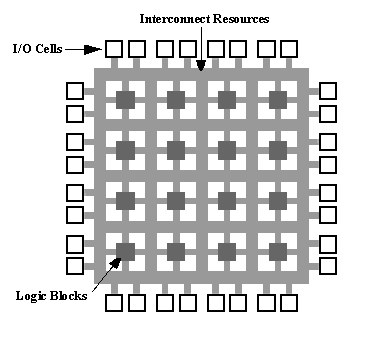
\includegraphics[width=0.5\textwidth,keepaspectratio=true]{./images/fpga1a}
 % \caption{Componentes de una FPGA}
  \label{fig:esquema}
 \end{center}
\end{figure}


%Conclusión!!Trabajar con un sistema final bajo licencias de hardware siguiendo el modelo de la Licencia LGPL para el software. Estamos comprometidos con el ideal de libre disposición, de libre uso y hardware de código abierto reutilizable.


